
\section{Introduction}
\begin{frame}[c]
  \frametitle{Motivation}
  \ldots clay repos\ldots 
\end{frame}

\begin{frame}[c]
  \frametitle{Clay Generic Disposal System Model}
Sensitivity analysis was performed with respect to various key processes and 
parameters affecting long-term post-closure performance of geologic repositories 
in clay media. 

Based on the detailed computational Clay 
\gls{GDSE} developed by the \gls{UFD} campaign \cite{clayton_generic_2011}, 
these results provide an overview of the relative importance of processes 
that affect the repository performance of a generic clay disposal concept model. 
\end{frame}


\begin{frame}[c]
  \frametitle{Clay Generic Disposal System Model}
The Clay \gls{GDSM} is built on the GoldSim simulation framework and contaminant 
transport model.  This radionuclide transport toolset simulates chemical and 
physical attenuation processes including radionuclide solubility, dispersion 
phenomena, and reversible sorption \cite{golder_goldsim_2010, 
golder_goldsim_ct_2010}. Model input parameters supporting modeling of these 
tranport 
processes include geometry specifications (e.g. repository depth), geologic 
material properties (e.g. clay porosity), geochemical data 
(e.g. elemental solubility limits), and environmental parameters (e.g. natural 
system velocity). Probabilistic elements of the GoldSim modeling 
framework enable the models to incorporate simple probabilistic \gls{FEPs} that 
affect repository performance.
\end{frame}

\begin{frame}[c]
  \frametitle{Clay Generic Disposal System Model}
\begin{figure}[htb!]
\begin{center}
\includegraphics[width=\linewidth]{feps.eps}
\end{center}
\caption{\ref{clayton_generic_2011}}
\label{fig:feps}
\end{figure}
\end{frame}

\begin{frame}[c]
  \frametitle{Clay Generic Disposal System Model}
The disposal concept modeled by the Clay \gls{GDSM} is an array of spent nuclear 
fuel packages within a clay repository envrionment, 500 meters beneath the 
earth's surface. In this repository concept, the waste packages contain an 
inventory of spent nuclear fuel, are emplaced horizontally in excavated tunnels, 
and are backfilled by a reducing bentonite clay buffer material within the 
tunnel \cite{nutt_generic_2009}. 

In the \gls{UFD} \gls{GDSM} tool that was used for this analysis, the clay 
repository concept is modeled using a single rectangular disposal cell. The 
disposal cell models a single cylindrical spent nuclear fuel package surrounded 
by bentonite buffer material and emplaced in the clay geologic medium. Using 
reflective boundary conditions in the horizontal plane, an infinite disposal 
cell array is modeled \cite{clayton_generic_2009}.

The model includes vertical advective fast pathway as well as an \gls{EBS} which 
can undergo rate based dissolution and barrier failure.  Releases from the 
\gls{EBS} enter near field and subsequently far field host rock regions in which 
diffusive and advective transport take place, attenuated by solubility limits as 
well as sorption and dispersion phenomena \cite{clayton_generic_2011}.
\end{frame}

\begin{frame}[c]
  \frametitle{Mean of the Peak Annual Dose}
In this analysis, repository performance is quantified by radiation dose to a 
hypothetical receptor. Specifically, this sensitivity analysis focuses 
on parameters that affect the mean of the peak annual dose.  The mean of the 
peak annual dose,

\begin{align} \label{MoP}
  D_{MoP,i} &= \frac{\sum_{r=1}^{N}{\max\left[\left.D_{r,i}(t)\right|_{\forall t}\right]}}{N}
  \intertext{where}
  D_{MoP,i} &= \mbox{ mean of peak annual dose due to isotope i } [mrem/yr]\nonumber\\
  D_{r,i}(t) &= \mbox{ year t dose in realization r due to isotope i } [mrem/yr]\nonumber\\
  N &= \mbox{number of realizations, } \nonumber
\end{align}

is a conservative metric of repository performance and should not be confused 
with the peak of the mean annual dose.

%\begin{align} \label{PoM}
%  D_{PoM,i} &= \max\left[{\frac{\sum_{r=1}^{N}{\left.D_{r,i}(t)\right|_{\forall t}}}{N}}\right]\\
%            &= \mbox{peak of the mean annual dose due to isotope i } [mrem/yr].\nonumber
%\end{align}
\end{frame}

\begin{frame}[c]
  \frametitle{Sampling Strategy}
This analysis has undertaken an analysis strategy to develop a many dimensional 
overview of the key factors in modeled repository performance. To achieve this, 
both individual and dual parametric cases were performed.

Individual parameter cases varied a single parameter of interest in 
detail over a broad range of values. Dual parameter cases were 
performed for pairs of parameters expected to exhibit some covariance. For 
each parameter or pair of parameters, forty simulation 
groups varied the parameter or parameters within the range considered. Each 
case and its parametric range are detailed in Table \ref{tab:Cases}. 

\begin{table}[ht!]
\centering
\footnotesize{
\begin{tabular}{|l|l|l|r|r|}
\multicolumn{5}{c}{\textbf{Simulation Cases}}\\
\hline
\textbf{Case} & \textbf{Parameter} & \textbf{Units} & \textbf{Min. Value} & \textbf{Max. Value}\\
\hline
V     & $R_{WFDeg.}$           & $[yr^{-1}]$       & $10^{-9}$    &  $10^{-2}$ \\
      & Inventory              & [MTHM]         & $10^{-4}$    &  $10^1$ \\
\hline
\end{tabular}
\caption{Each dual and single parameter simulation case had 40 simulation 
groups of 100 realizations each.}
\label{tab:Cases}
}
\end{table}



For each simulation group, a 100 realization simulation was completed. Each
realization held the parameters being analyzed as constant and sampled 
stochastic values for uncertain parameters not being studied.  A sampling scheme 
developed in previous generic disposal media modeling was implemented in this 
model in order to ensure that the each 100 realization simulation sampled 
identical values for uncertain parameters \cite{clayton_generic_2011, 
nutt_generic_2009}.  

\end{frame}
